\begin{frame}[parent={ie:agenda}, hasnext=true, hasprev=false]
	\frametitle{Modelo de Royce}

	\begin{block:concept}{Definição}
		Modelos para produção de programas grandes (e erroneamente associado com a
		criação do modelo cascata)~\cite{Royce:1970}.
	\end{block:concept}
	
	\begin{block:fact}{Contexto}
		\begin{itemize}
			\item Projetos para desenvolvimento de software para planejamento,
			comando e análise pós-vôo de missões espaciais.
					
			\item \~ 1960.
		\end{itemize}
	\end{block:fact}
	
	\note{
		\begin{itemize}
			\item Erroneamente atribuído como criador do Modelo Cascata.
			
			\item Curiosidade: o filho mais velho de Winston Royce, Walker
			Royce, foi um dos responsáveis pelo RUP (Rational Unified
			Process).
		\end{itemize}
	}
\end{frame}


\begin{frame}[hasnext=true, hasprev=true]
	\frametitle{Modelo de Royce}

	\begin{block:fact}{Modelo Cascata}
		\centering
		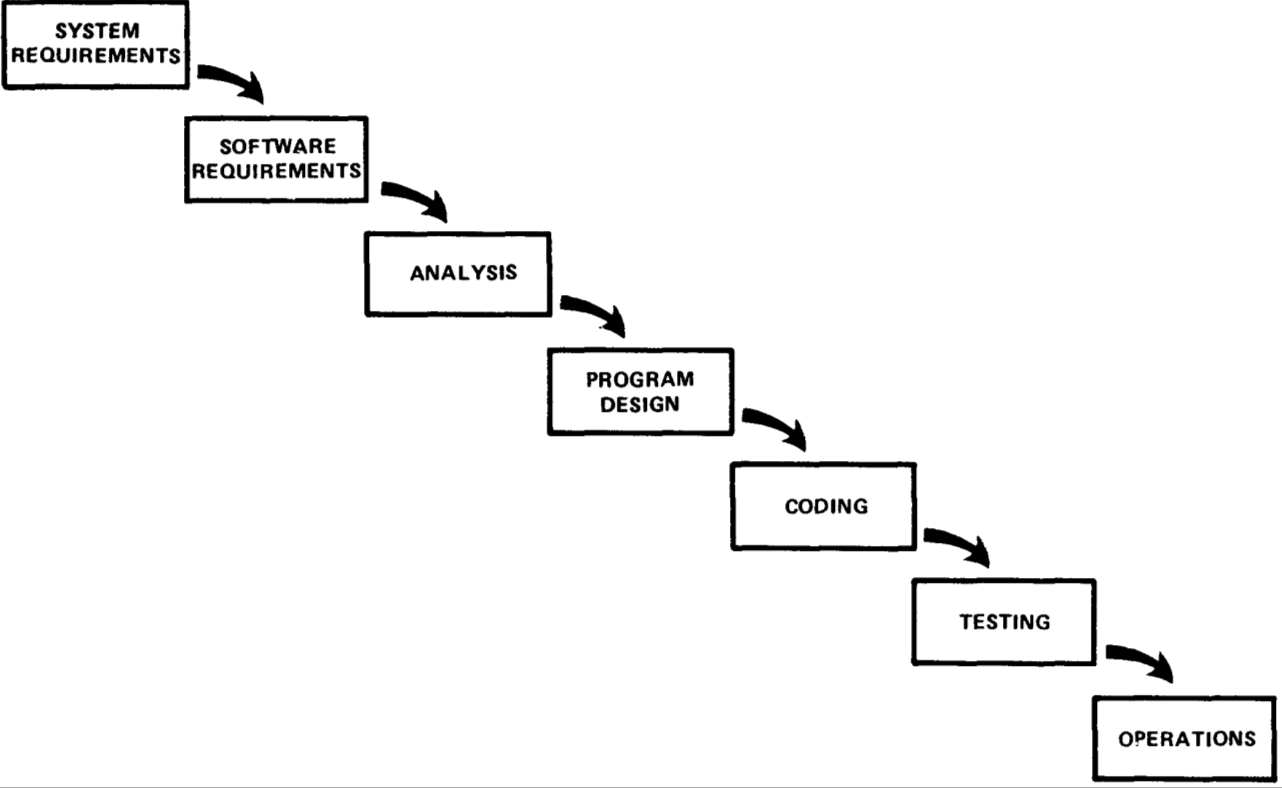
\includegraphics[width=\textwidth]{software-engineering/project-management/process/sdlc/royce/waterfall}
	\end{block:fact}
	
	\note{
		\begin{itemize}
			\item Modelo que inclua apenas análise e codificação está fadado ao
			fracasso para projetos grandes.
			
			\item Para ser bem sucedido, deve incluir mais níveis de análise de
			requisitos, um nível de projeto e um para teste de software.
		\end{itemize}
	}
\end{frame}


\begin{frame}
	\frametitle{Modelo de Royce}

	\begin{block:fact}{Modelo Cascata com iterações entre as fases}
		\centering
		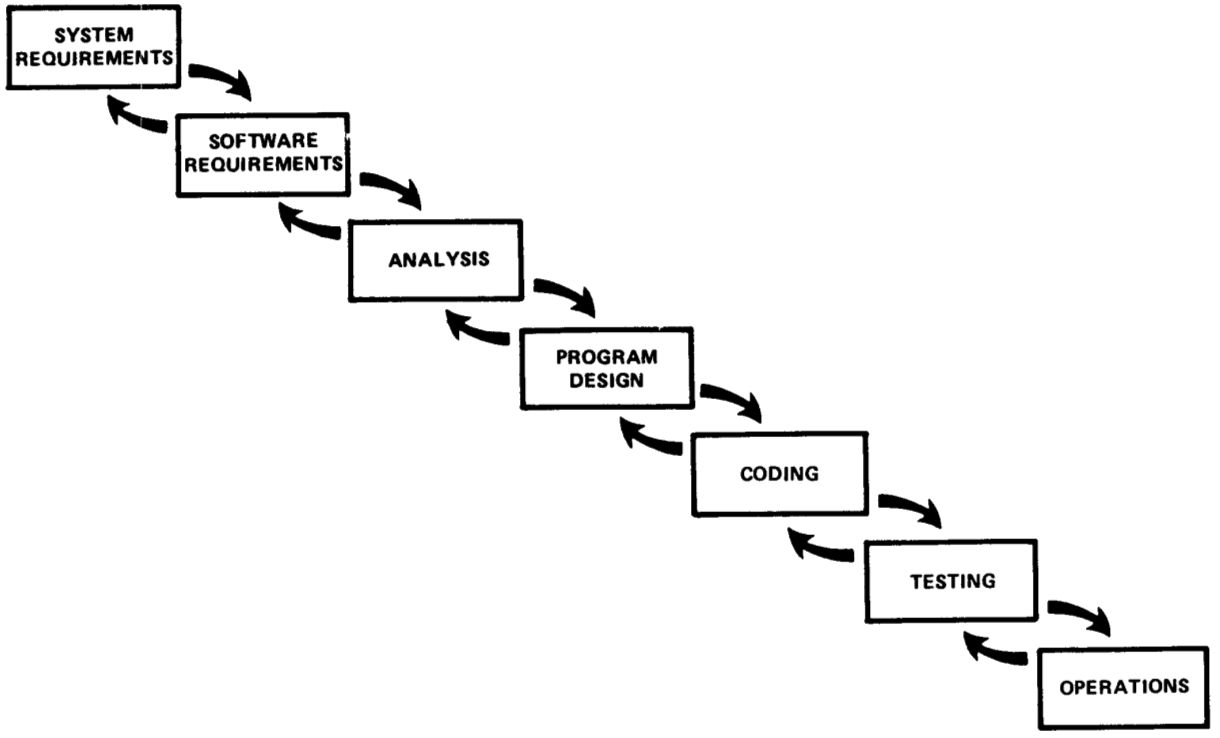
\includegraphics[width=\textwidth]{software-engineering/project-management/process/sdlc/royce/iterative-waterfall}
	\end{block:fact}
	
	\note{
		\begin{itemize}
			\item Existe iteração entre as fases imediatamente vizinhas e, raramente,
			com fases mais distantes.
			
			\item Com as iterações existe uma tentativa de maximizar o trabalho feito
			e que pode ser salvo/preservado.
		\end{itemize}
	}
\end{frame}


\begin{frame}
	\frametitle{Modelo de Royce}

	\begin{block:fact}{Modelo Cascata com reprojeto}
		\centering
		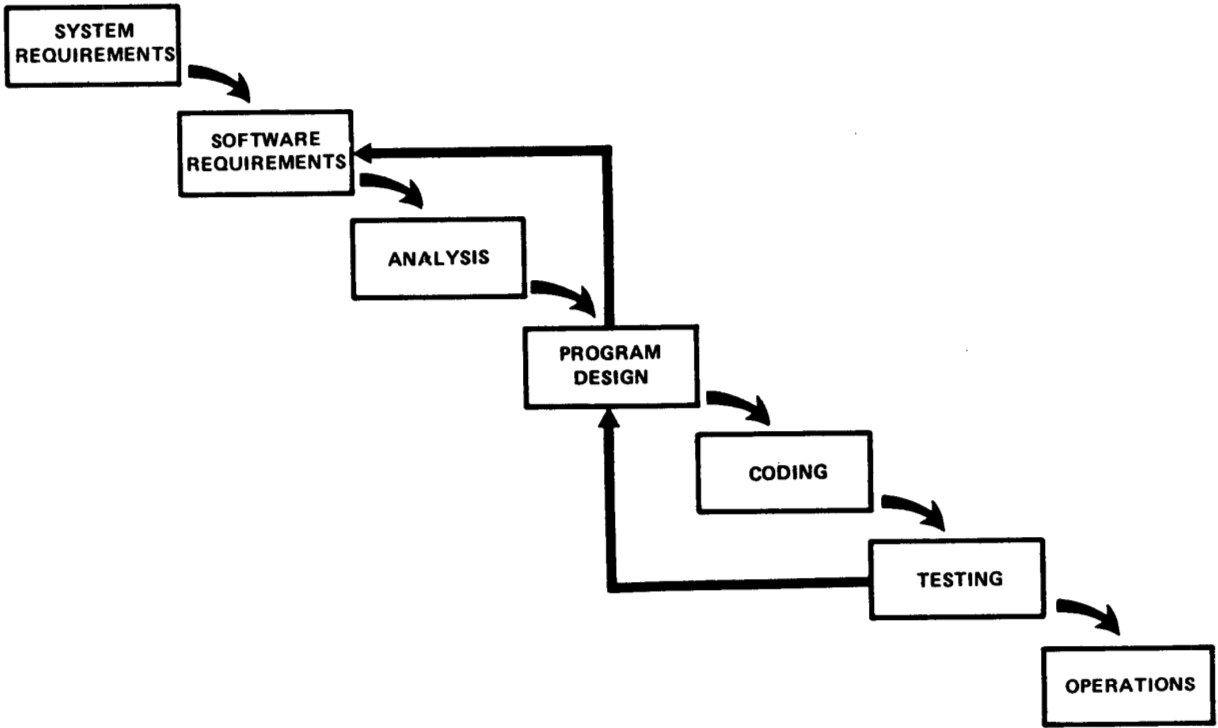
\includegraphics[width=\textwidth]{software-engineering/project-management/process/sdlc/royce/alternative-waterfall}
	\end{block:fact}
	
	\note{
		\begin{itemize}
			\item Erros no teste podem causar a mudança do projeto do software ou ainda
			dos próprios requisitos.
			
			\item As bases de codificação e análise são pulados porque elas são mais
			fáceis de gerenciar (ao menos nos projetos do contexto do Royce).
			
			\item Todavia, nenhum desses modelos é razoável para Royce\ldots
		\end{itemize}
	}
\end{frame}


\begin{frame}[hasnext=false, hasprev=true]
	\frametitle{Modelo de Royce}

	\begin{block:fact}{}
		\centering
		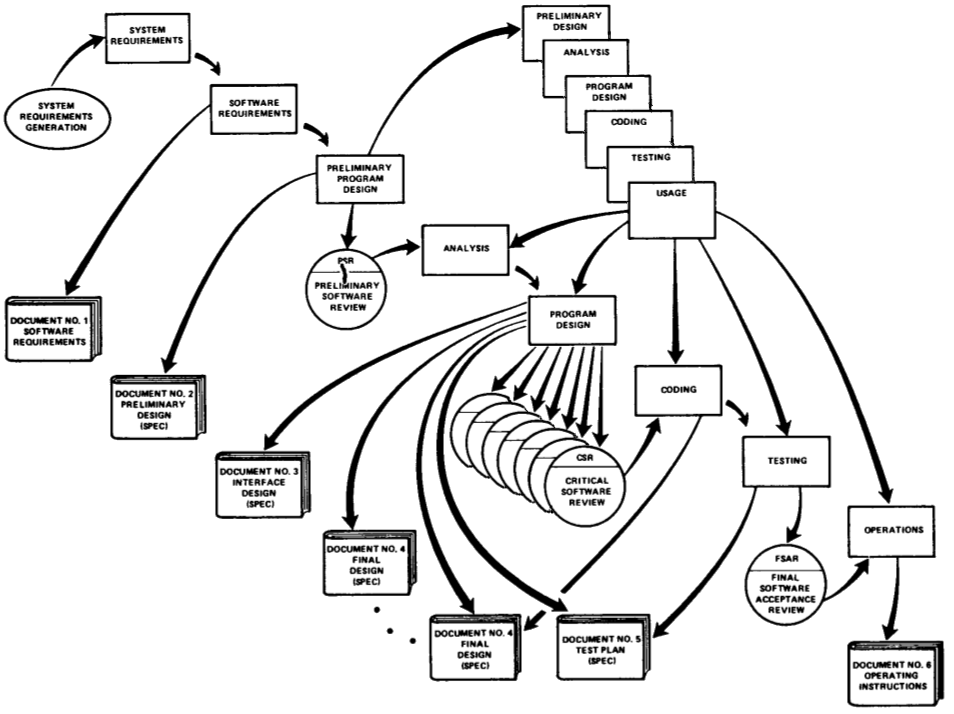
\includegraphics[width=\textwidth]{software-engineering/project-management/process/sdlc/royce/royce-model}
	\end{block:fact}
	
	\note{
		\small
		\begin{itemize}
			\item Complete o projeto do programa antes de iniciar a análise.
			\begin{itemize}
				\small
				\item Melhor identificar os problemas no início do que no final.
			\end{itemize}
			
			\item Documentação deve sempre estar atualizada e completa.
			\begin{itemize}
				\small
				\item Essencial para tomar decisões gerenciais.
			\end{itemize}
			
			\item Faça o trabalho duas vezes se possível (principalmente se for a
			primeira versão do produto).
% 			\begin{itemize}
% 				\small
% 				\item Uma iteração curta (1/3 do tempo do projeto total) e outra iteração
% 				para produzir o produto final.
% 			\end{itemize}
			
			\item Teste deve ser planejado, controlado e monitorado.
			\begin{itemize}
				\small
				\item Teste pelo especialista de teste, utilizando critérios baseados em
				fluxo de controle.
				\item Fazer inspeção de software.
			\end{itemize}
			
			\item Envolva o cliente.
		\end{itemize}
	}
\end{frame}